\documentclass[a4paper,twoside]{article}

\usepackage{epsfig}
\usepackage{subfigure}
\usepackage{calc}
\usepackage{amssymb}
\usepackage{amstext}
\usepackage{amsmath}
\usepackage{amsthm}
\usepackage{multicol}
\usepackage{pslatex}
\usepackage{apalike}
\usepackage{SCITEPRESS}     % Please add other packages that you may need BEFORE the SCITEPRESS.sty package.

\usepackage{url}% http://ctan.org/pkg/url
\usepackage{flushend}

\subfigtopskip=0pt
\subfigcapskip=0pt
\subfigbottomskip=0pt

\begin{document}


\title{Enabling the Use of GPU Virtualization in Cloud Environments}
\author{\authorname{Sergio Iserte, Francisco J. Clemente-Castell\'o, Adri\'an Castell\'o,\\Rafael Mayo and Enrique S. Quintana-Ort\'i}
\affiliation{Department of Computer Science and Engineering\\Universitat Jaume I - Castell\'o de la Plana, Spain}
\email{\{siserte, fclement, adcastel, mayo, quintana\}@uji.es}}

\keywords{Cloud Computing, GPU Virtualization, Resource Management}

\abstract{The use of accelerators in order to reduce the execution time of some 
application has become more popular during last years. These devices increment 
the computational power of a node thanks to its parallel architecture. %The popularity of the GPGPU computation 
This trend has led several cloud vendors such as Amazon Web Services or some 
middlewares such as OpenStack to add to their current facilities, or to allow, 
instances of virtual machines equipped with NVIDIA GPUs. 
Accomplishing this requirements needs that the guest hosts must be equipped with 
GPUs which could be barely utilized if a non GPU-enabled Virtual Machine is running in the host.
The solution presented in this work is based on GPU virtualization and shareability 
in order to reach an equilibrium between supply and demand of accelerators from the users. 
Hence, we propose to decouple from the nodes, real GPUs by using the virtualization technology called rCUDA. 
With this software configuration, these GPUs can be accessed from any VM getting rid 
of the necessity of having physical GPUs in the guest host. 
Moreover, our project studies the viability of these join by using a public cloud 
service configuration and develops a module for OpenStack middleware in order to 
add the needed support for the virtualized devices and the logic to manage them. 
The results show a feasible configuration which adds flexibility to the current and well-known 
cloud solutions. 
}

\onecolumn \maketitle \normalsize \vfill

\section{\uppercase{Introduction}}
\label{sec:introduction}

%\noindent 


\section{\uppercase{Background}}
\label{sec:background}
\subsection{The rCUDA Framework}
\label{sec:rcuda}

{rCUDA}~\cite{tonithesis,toniparco} is a middleware that enables transparent access
to any NVIDIA GPU device present in a cluster from all compute
nodes. The GPUs can be accessed and shared between nodes, and a single node can use all these graphic accelerators
as if they were local.
These features are focused in attaining higher accelerator utilization rates in the overall system while simultaneously reducing
resource, space, and energy~\cite{energy14} requirements.
rCUDA is structured following a client-server distributed
architecture: the client middleware is allocated in the same cluster node where the application demanding GPGPU
acceleration services is executed, providing a transparent replacement for the
native CUDA libraries. Furthermore, the server middleware is executed in the
cluster nodes from which the actual GPUs provide the requested GPGPU service.
To support a concurrent scenario where GPUs are shared between
processes\slash nodes, {rCUDA} manages separate device contexts for
each client application.

The {rCUDA} 5.0 client exposes the same interface as the regular NVIDIA
CUDA 6.5 release~\cite{cuda65}, including the runtime and driver
APIs as well as other commonly used libraries such as cuBLAS, cuFFT, cuSparse or cuRand.
Therefore, applications are not aware of the fact that they are being executed
on top of a virtualization layer.
With the aim to be updated with new GPU programming models, {rCUDA} also supports
directive-based models such as OmpSS~\cite{repara15} and OpenACC~\cite{cluster15}.

The integration of remote GPGPU virtualization with global
resource schedulers such as SLURM~\cite{sbacpad14} completes this powerful
technology, making accelerator-enabled clusters more flexible and
energy efficient.

\subsection{Amazon Web Services}
\label{sec:aws}
AWS~\cite{aws} is a public cloud computing provider
and it is composed by several cloud services such as 
 cloud-based computation, storage and other functionality 
that enables organizations and/or individuals to deploy
services and applications on an on-demand basis. 
These services, replace IT infrastructure for most companies, and provide agility and instant elasticity matching 
perfectly with their software requirements.

From the point of view of HPC, AWS offers high performance facilities including 
instances equipped with GPUs and high performance network interconnection which 
are common resources used in this research field.

\subsection{OpenStack}
\label{sec:openstack}

OpenStack~\cite{OpenStack} is a cloud operating system that provides Infrastructure as a Service (IaaS). 
It is able to control large pools of compute, storage, and networking resources throughout a 
datacenter. All these resources are managed through a dashboard or an API that gives administrators 
control while empowering their users to provision resources through a web interface
or a command-line. 
It supports most available hypervisors and handles provisioning 
and life-cycle management of VMs.
 
The OpenStack architecture offers a flexibility to create a custom cloud, with no proprietary hardware
or software requirements and the ability to integrate with legacy systems and third party technologies. 

From the HPC perspective, OpenStack offers high performance computing (HPC) configurations using
multiple supported hypervisors and different hardware architectures. However, despite to be able to
specify some extra parameters for special resources like GPUs, choosing a host based on the existence
of a GPU is currently unsupported in OpenStack~\cite{OpenStackGPU}. 

\section{\uppercase{State of Art}}
\label{sec:state}
Our solutions
is based on GPU virtualization and sharing resources in order
to reach a fair balance between supply and demand.
Several attempts of achieving what we are pursing have been
made, but none of them are so ambitious as our project. On
the one hand the work done in~\cite{younge2013enabling} allows the VM managed
by the hypervisor Xen to access the GPUs in the physical
node. With the implied limitations of restricting the nodes not
to use more GPUs than the hosted in the machine and not
to share idle GPUs to other machines. The solution presented
by the project gVirtus~\cite{giunta2010gpgpu} does virtualize GPUs and make
them accessible for any VM in the cluster. However, this kind
of virtualization strongly depends on the hypervisor used, so
does its performance. Another similar solution is presented in~\cite{diab2013dynamic} by the name of gCloud. This one continues without being
integrated in a Cloud Computing Manager, though its main
drawback is that the code of the applications must be modified
in order to be run in their virtual-GPU environment. On the
other hand, the work exposed in~\cite{jungpgpu} is more mature, however,
it is only focussed on compute intensive HPC applications.
The main idea of our proposal goes further and apart from
bringing solutions for all kind of HPC applications, it is aimed
to boost the cluster flexibility in the use of GPUs.

\section{\uppercase{Motivation}}
\label{sec:motivation}

Cloud computing, storage and other facilities are becoming 
more popular during the last years thanks to the easy set up 
process and the low required IT invest. The features provided 
by the cloud vendors are useful for companies and individuals 
which have access to the last technology without spending a 
huge amount of money. Moreover, the systems offered by the cloud 
companies matches with the ones required thanks to its flexibility.

The power of current cloud vendors is based on the use 
of Virtual Machines (VM) which  
emulates a physical node with its own 
CPUs, storage, network interconnection, OS and GPU. 
However, to provide a VM with GPUs means
that the guest host must be equipped with at least one GPU, and
once it has been assigned to an instance, no other VM can use
it. Therefore, the number of VM that are allowed to use a GPU is 
limited by the number of the installed devices. This lack of 
flexibility is also noticed in the cluster configurations, where 
depending on the users’ necessities, 
two approaches to introduce GPGPU computation can be determined:
the conservative, to have a lot of hosts with GPUs to be
ensured that you are likely to satisfy all the requests; or a
more daring approach, where you will count with some GPU-
enabled nodes hoping not to arrive a large burst of requests
so the cluster would run out of GPU resources.

The use of a virtualization technology such as {rCUDA} adds 
the desired flexibility because this software detaches the GPUs 
from the nodes where they are installed allowing all nodes in a cluster
not only use them as if they were local but also to share them 
achieving a higher utilization rate and reducing the idle status time.

Thanks to the shareability introduced by {rCUDA}, all VM in the cloud 
environment should be able to use and share all the GPUs installed in 
the physical nodes removing the current limitation. But, in order to achieve this goal, 
the cloud facilities need to be provided with the {rCUDA} software and 
in the case of OpenStack, a module for manageing virtualized GPUs 
 has to be implemented.  



\section{\uppercase{Working with AWS}}
\label{sec:aws}
In this section, first of all, the current user-level features 
provided by the Amazon Web Services are explained and analyzed 
from the point of view of the GPU usage. 
Finally, the scenarios and experiments where virtualized GPUs are utilized are 
described and first results are showed.

\subsection{Current Features}
This subsection explains the most common features checked during 
the virtual machine creation step.

\subsubsection{Instances}

An instance is a pre-configured virtual machine focused on an 
specific target. Inside the large list of instances offered by AWS, 
we can find: general pourpose (T2, M4 and M3); computer science optimized 
(C4 and C3); memory optimized (R3); storage optimized (I2 and D2) and 
GPU capable instances. Each kind of instance has its own pourpose and its 
own price. Moreover, each instance has different number of CPUs and network 
interconnection which can be: low, medium, high or 10Gb.

For this study, the instances presented in the Table~\ref{table:awsInstances} 
have been selected. The C3 family instances, which are not equipped with 
GPUs are going to be used as client whereas the instances of the G2 family are 
acting as servers.   

\begin{table}[htb]
\renewcommand{\arraystretch}{1.3}
\caption{AWS available HPC instances.}
\label{table:awsInstances}
\tabcolsep=0.09cm
\begin{center}\begin{tabular}{cccccc}
Name & vCPUs & Memory & Network & GPUs & Price\\ \hline \hline
c3.2xlarge & 8 & 15 GiB & High & 0 & \$ 0.21\\ \hline
c3.8xlarge & 32 & 60 GiB & 10 Gb & 0 & \$ 1.68 \\ \hline
g2.2xlarge & 8 & 15 GiB & High & 1 & \$ 0.65\\ \hline
g2.8xlarge & 32 & 60 GiB & 10 Gb & 4 & \$ 2.6 \\ \hline
\end{tabular}\end{center}\end{table}

\subsubsection{Network behaviour}
As it is shown in the Table~\ref{table:awsInstances}, each instance has different 
interconnection and taking into account that the use of the network 
is critical when GPU virtualization is applied, a simple test to verify the 
real network bandwidth is needed.

\begin{table}[htb]
\renewcommand{\arraystretch}{1.3}
\caption{IPERF results between instances.}
\label{table:iperf}
\tabcolsep=0.24cm
\begin{center}\begin{tabular}{cccc}
Server & Client & Network & Bandwidth\\ \hline \hline
g2.8xlarge & c3.2xlarge & High & 1  Gb/s\\ \hline
g2.8xlarge & c3.8xlarge & 10Gb & 7.5  Gb/s\\ \hline
g2.8xlarge & g2.2xlarge & High & 1 Gb/s\\ \hline
g2.8xlarge & g2.8xlarge & 10Gb & 7.5  Gb/s\\ \hline
\end{tabular}\end{center}\end{table}

The IPERF tool has been executed between the instances showed in 
the Table~\ref{table:iperf} in order to know the real bandwidth.
Therefore, we can assure that the nomenclature ``High'' used in the 
network column correspond to a 1Gb interconnection and the 10Gb has 
a real bandwidth of 7.5Gb/s.
Moreover, it looks like the instances equipped with a ``High'' interconnection 
are software-limited up to 1 Gb/s due to the theoretical and real bandwith 
match perfectly. The gap between real and theorical can be observed with 
the 10Gb interconnection which reaches up to 7.5 Gb/s.


\subsubsection{GPUs}
As it has been said before, an instance is based in a VM 
which is running on a real node with its own virtualized 
components, so it is possible that AWS could use a virtualization 
framework to offer GPU services to all the instances.
Therefore, we need to verify if the GPUs showed in the instances are 
non-virtualized GPUs so, we have executed the NVIDIA SDK test called 
{\tt bandwidthtest}. As it is shown in the Table~\ref{table:bwt}, as the bandwidth achieved 
in this test is higher than the network bandwith, it reveals that it is a 
real GPU. 
\begin{table}[htb]
\renewcommand{\arraystretch}{1.3}
\caption{NVIDIA SDK {\tt bandwidthtest} execution transfering 32MB using pageable memory using local GPU.}
\label{table:bwt}
\tabcolsep=0.09cm
\begin{center}\begin{tabular}{cccc}
Name &  Data Movement & Network & BandWidth \\ \hline \hline
g2.2xlarge & Host to Device & High& 3,004 MB/s \\ \hline
g2.2xlarge & Device to Host & High& 2,809 MB/s\\ \hline
g2.8xlarge & Host to Device & 10 Gb& 2,814 MB/s\\ \hline
g2.8xlarge & Device to Host & 10 Gb& 3,182 MB/s\\ \hline
\end{tabular}\end{center}\end{table}

\subsection{Testbed Scenarios}
In this section, the different client-server configurations 
are explained. All the scenarios are based in the maximum number of instance 
that a user can freely select without submiting a formal request.

\begin{itemize}
\item Scenario A (Figure~\ref{subfig:aws1}) shows the most common 
and used hardware configuration in real clusters, where each node is 
populated with one GPU. Here, a simple node is able to use up to 5 GPUs 
using the ``High'' interconnection. 

\item Scenario B (Figure~\ref{subfig:aws2}) is composed by 2 server nodes equipped 
with 4 GPUs each one and a client that does not have any GPU. This scenario is using 
a 10Gb network and the cliend is able to execute application using up to 8 GPUs.

\item Scenario C (Figure~\ref{subfig:aws3}) joins both scenarios A and B. So a 
single client, using a 1Gb network interconnection, has 13 GPUs that can be used as if they were locally installed.
\end{itemize}

\begin{figure*}[ht]
\centering
\subfigure[5 remote GPUs over 1GbE.]{%
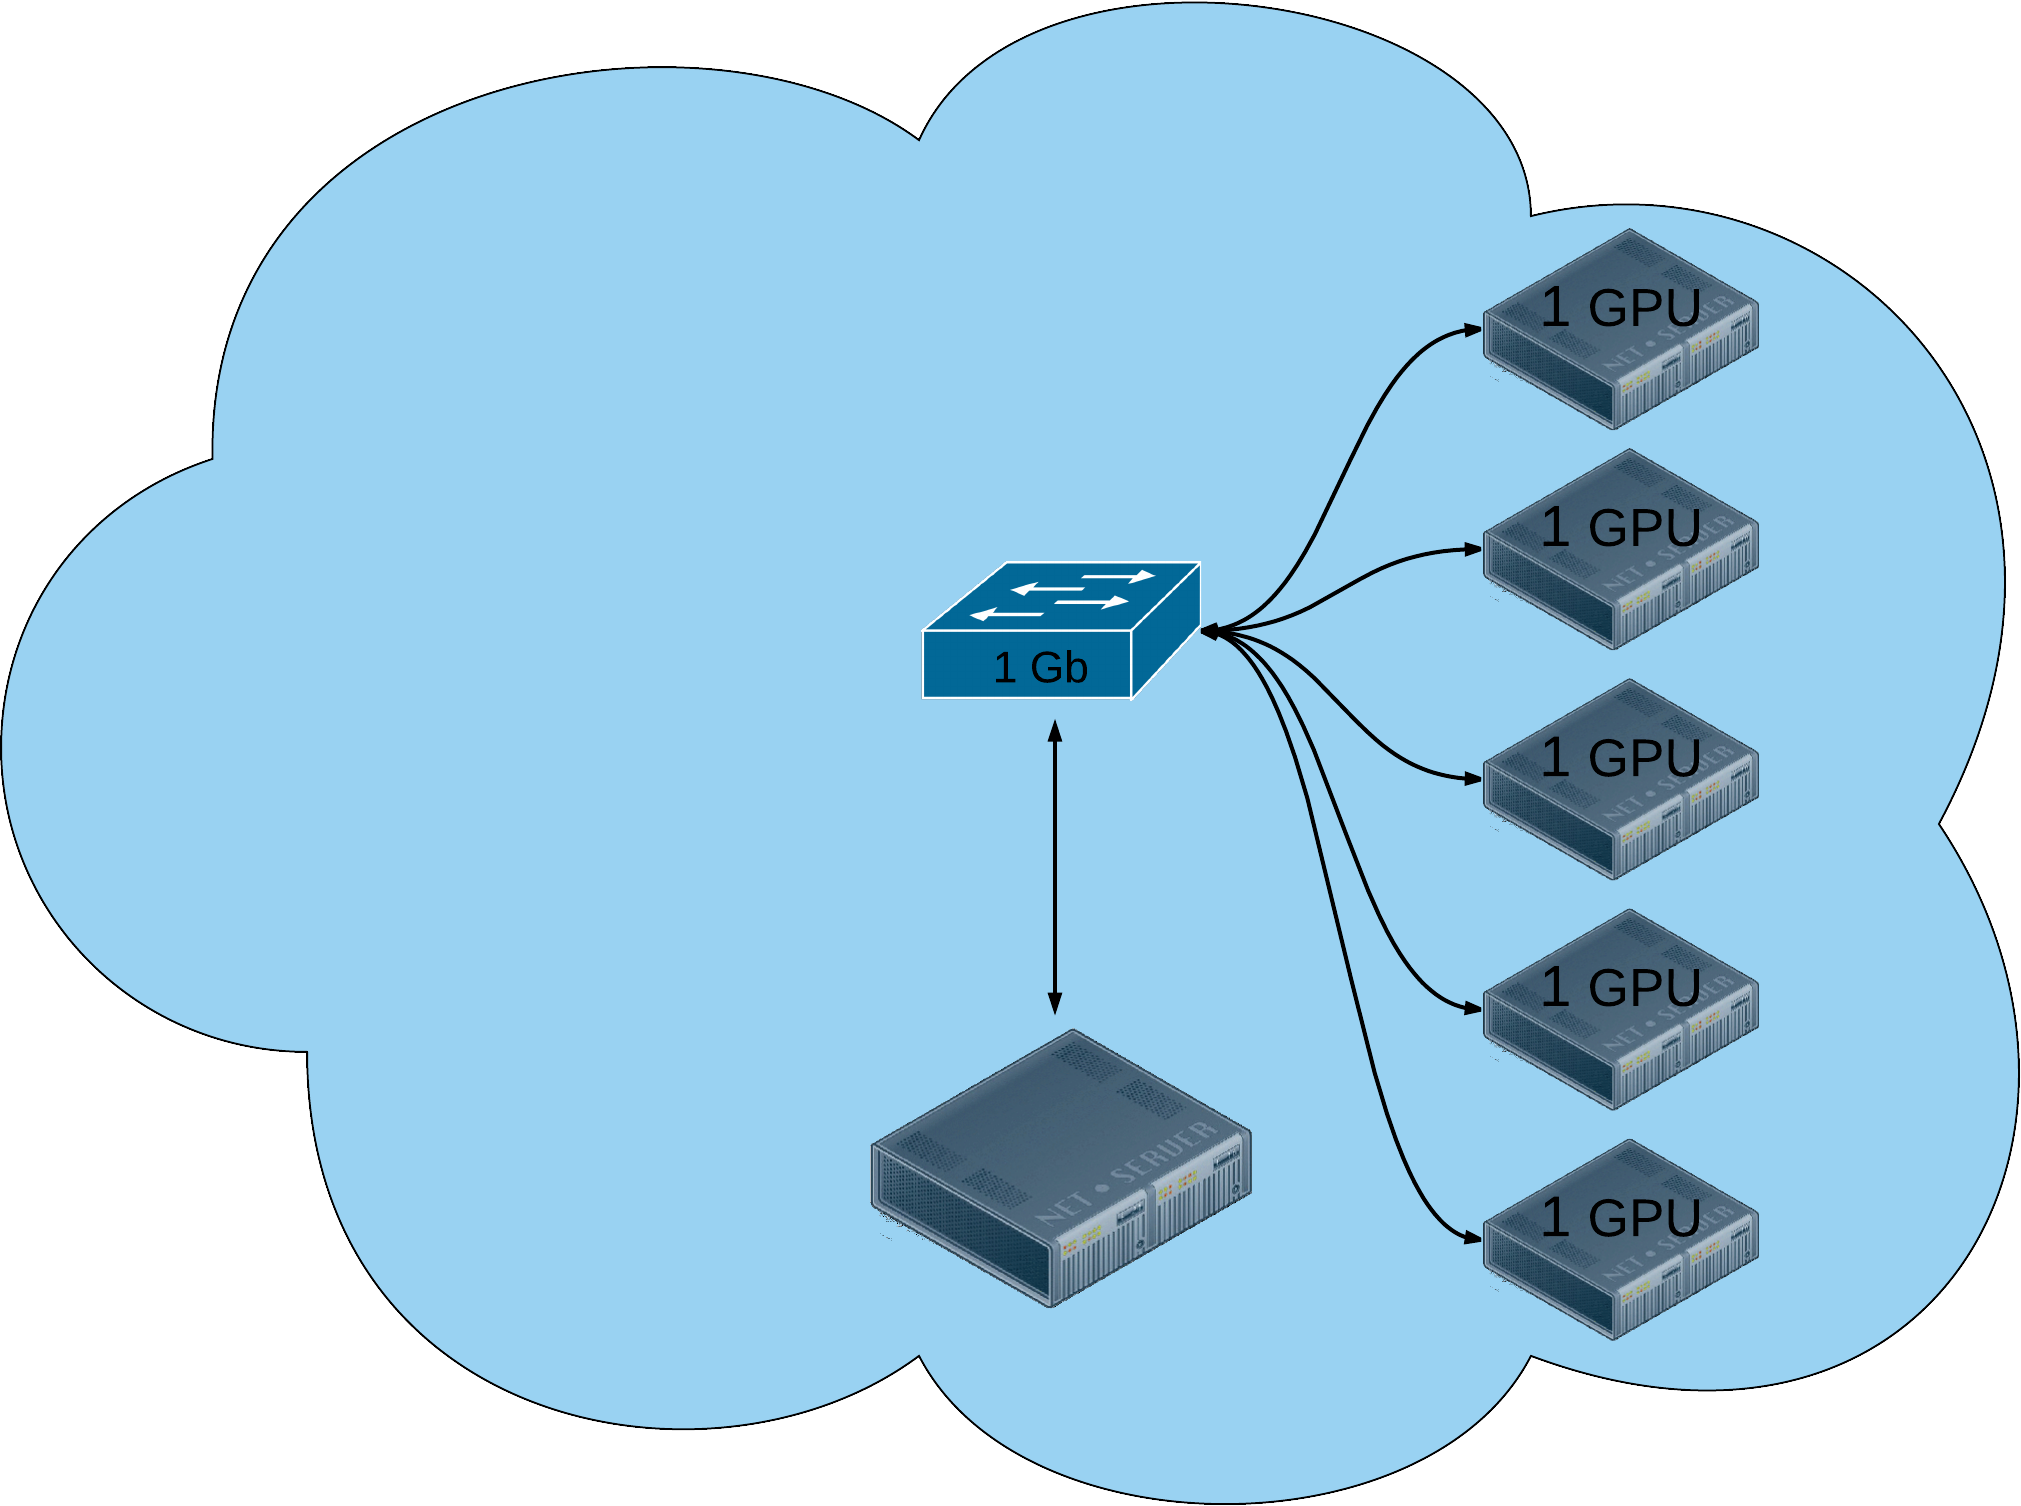
\includegraphics[width=0.31\linewidth]{images/aws3.png}
\label{subfig:aws1}}
\quad
\subfigure[8 remote GPUs over 10GbE.]{%
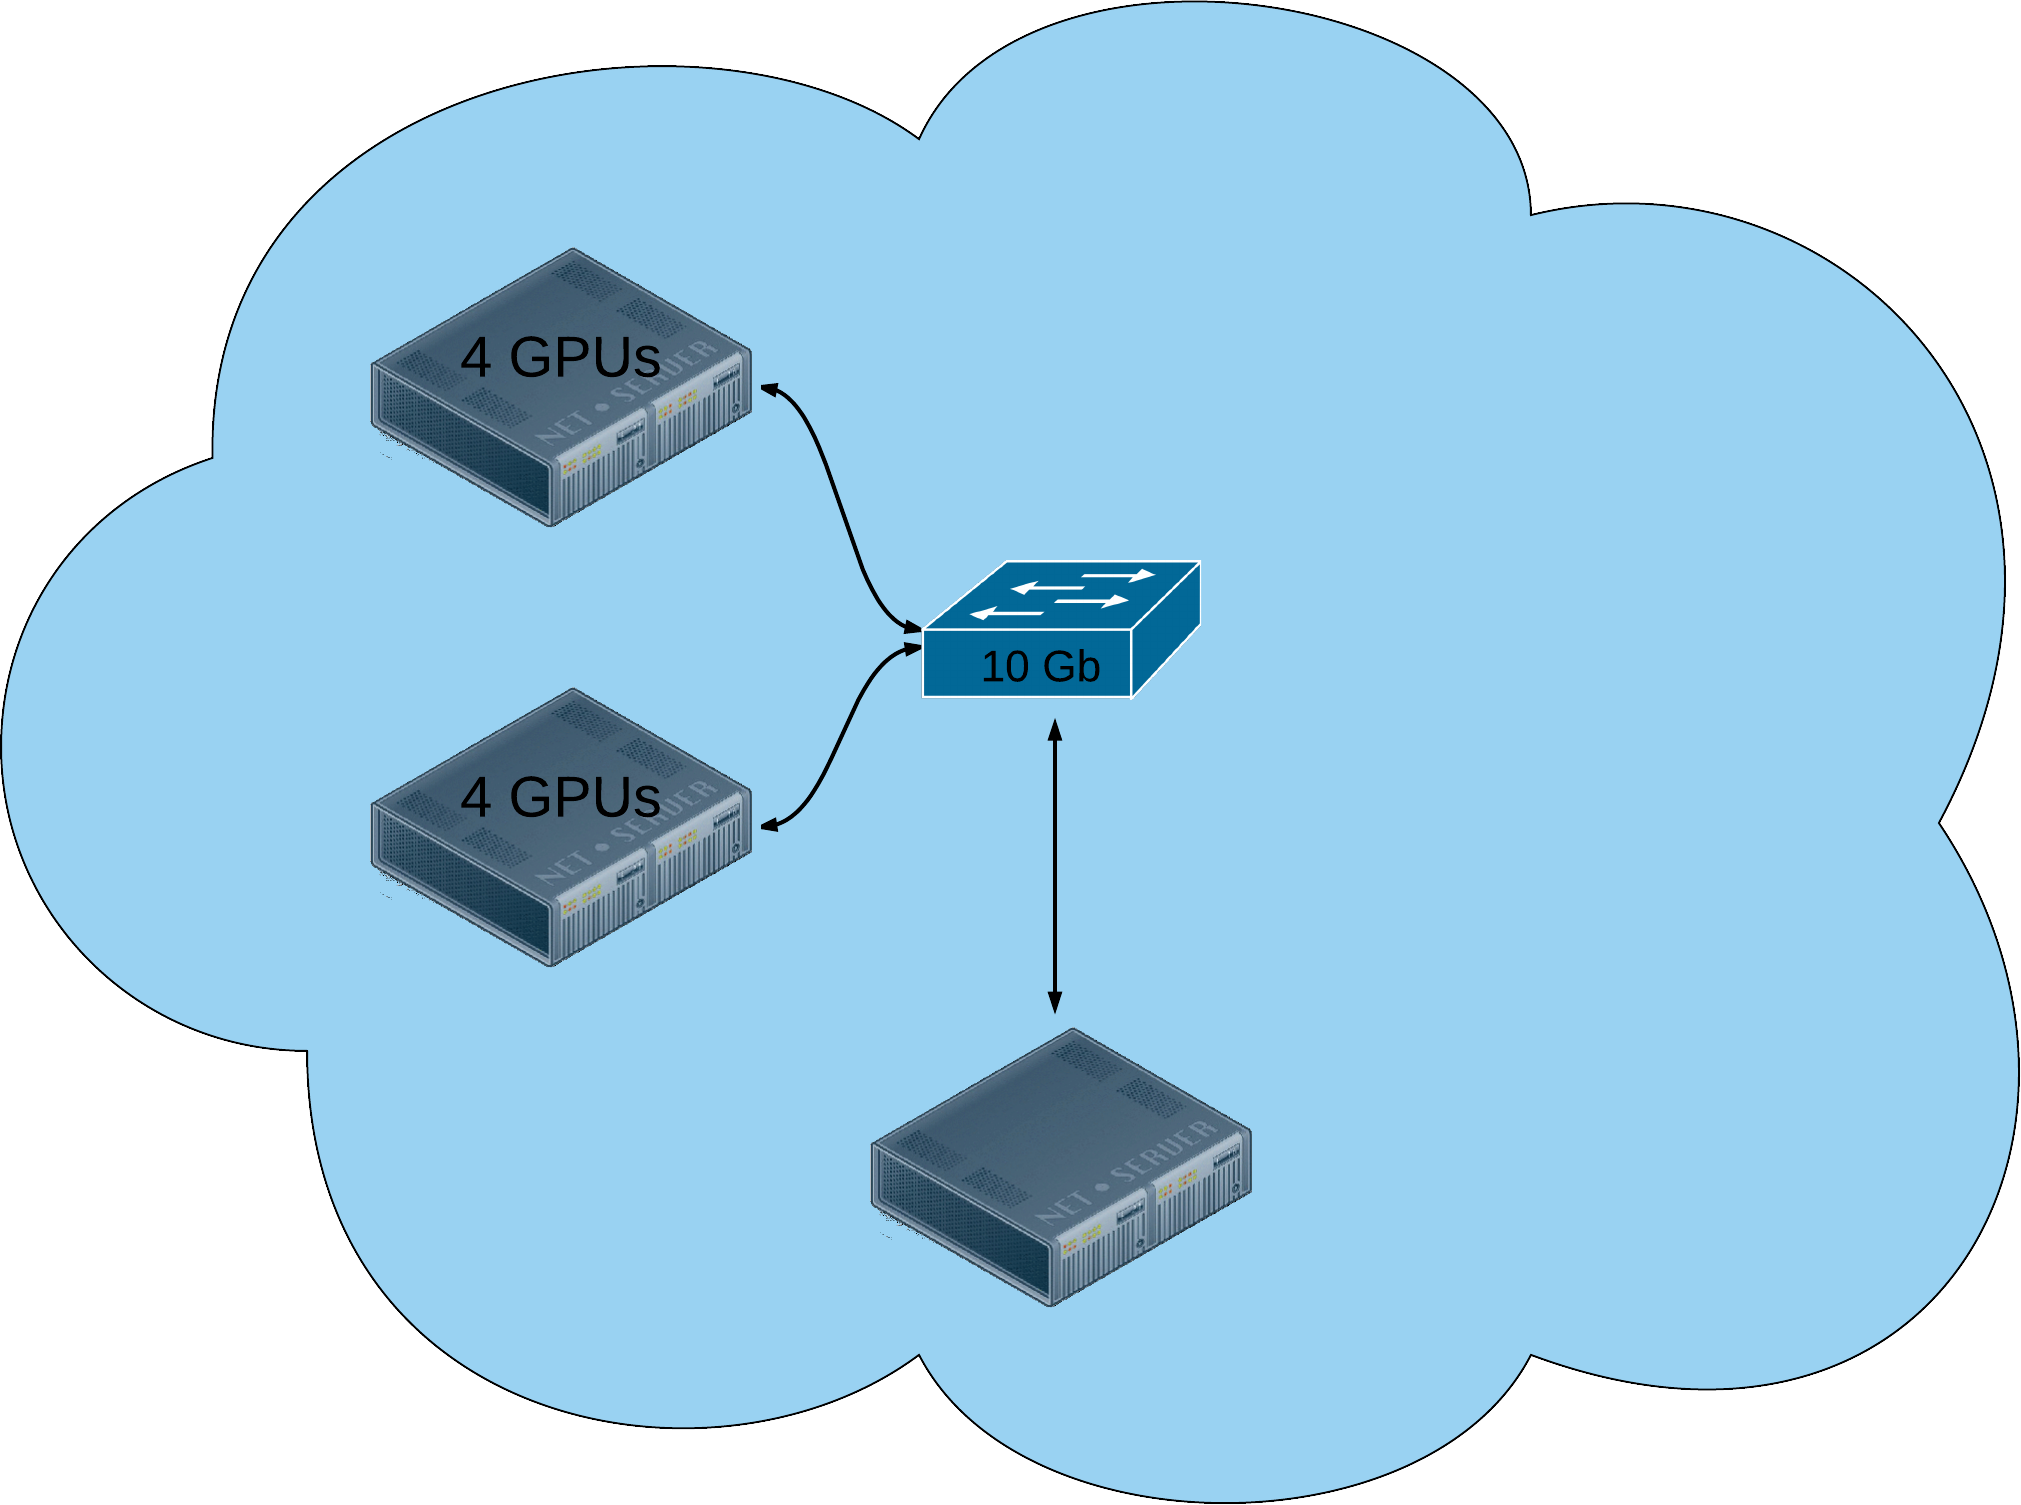
\includegraphics[width=0.31\linewidth]{images/aws2.png}
\label{subfig:aws2}}
\subfigure[13 remote GPUs over 1GbE.]{%
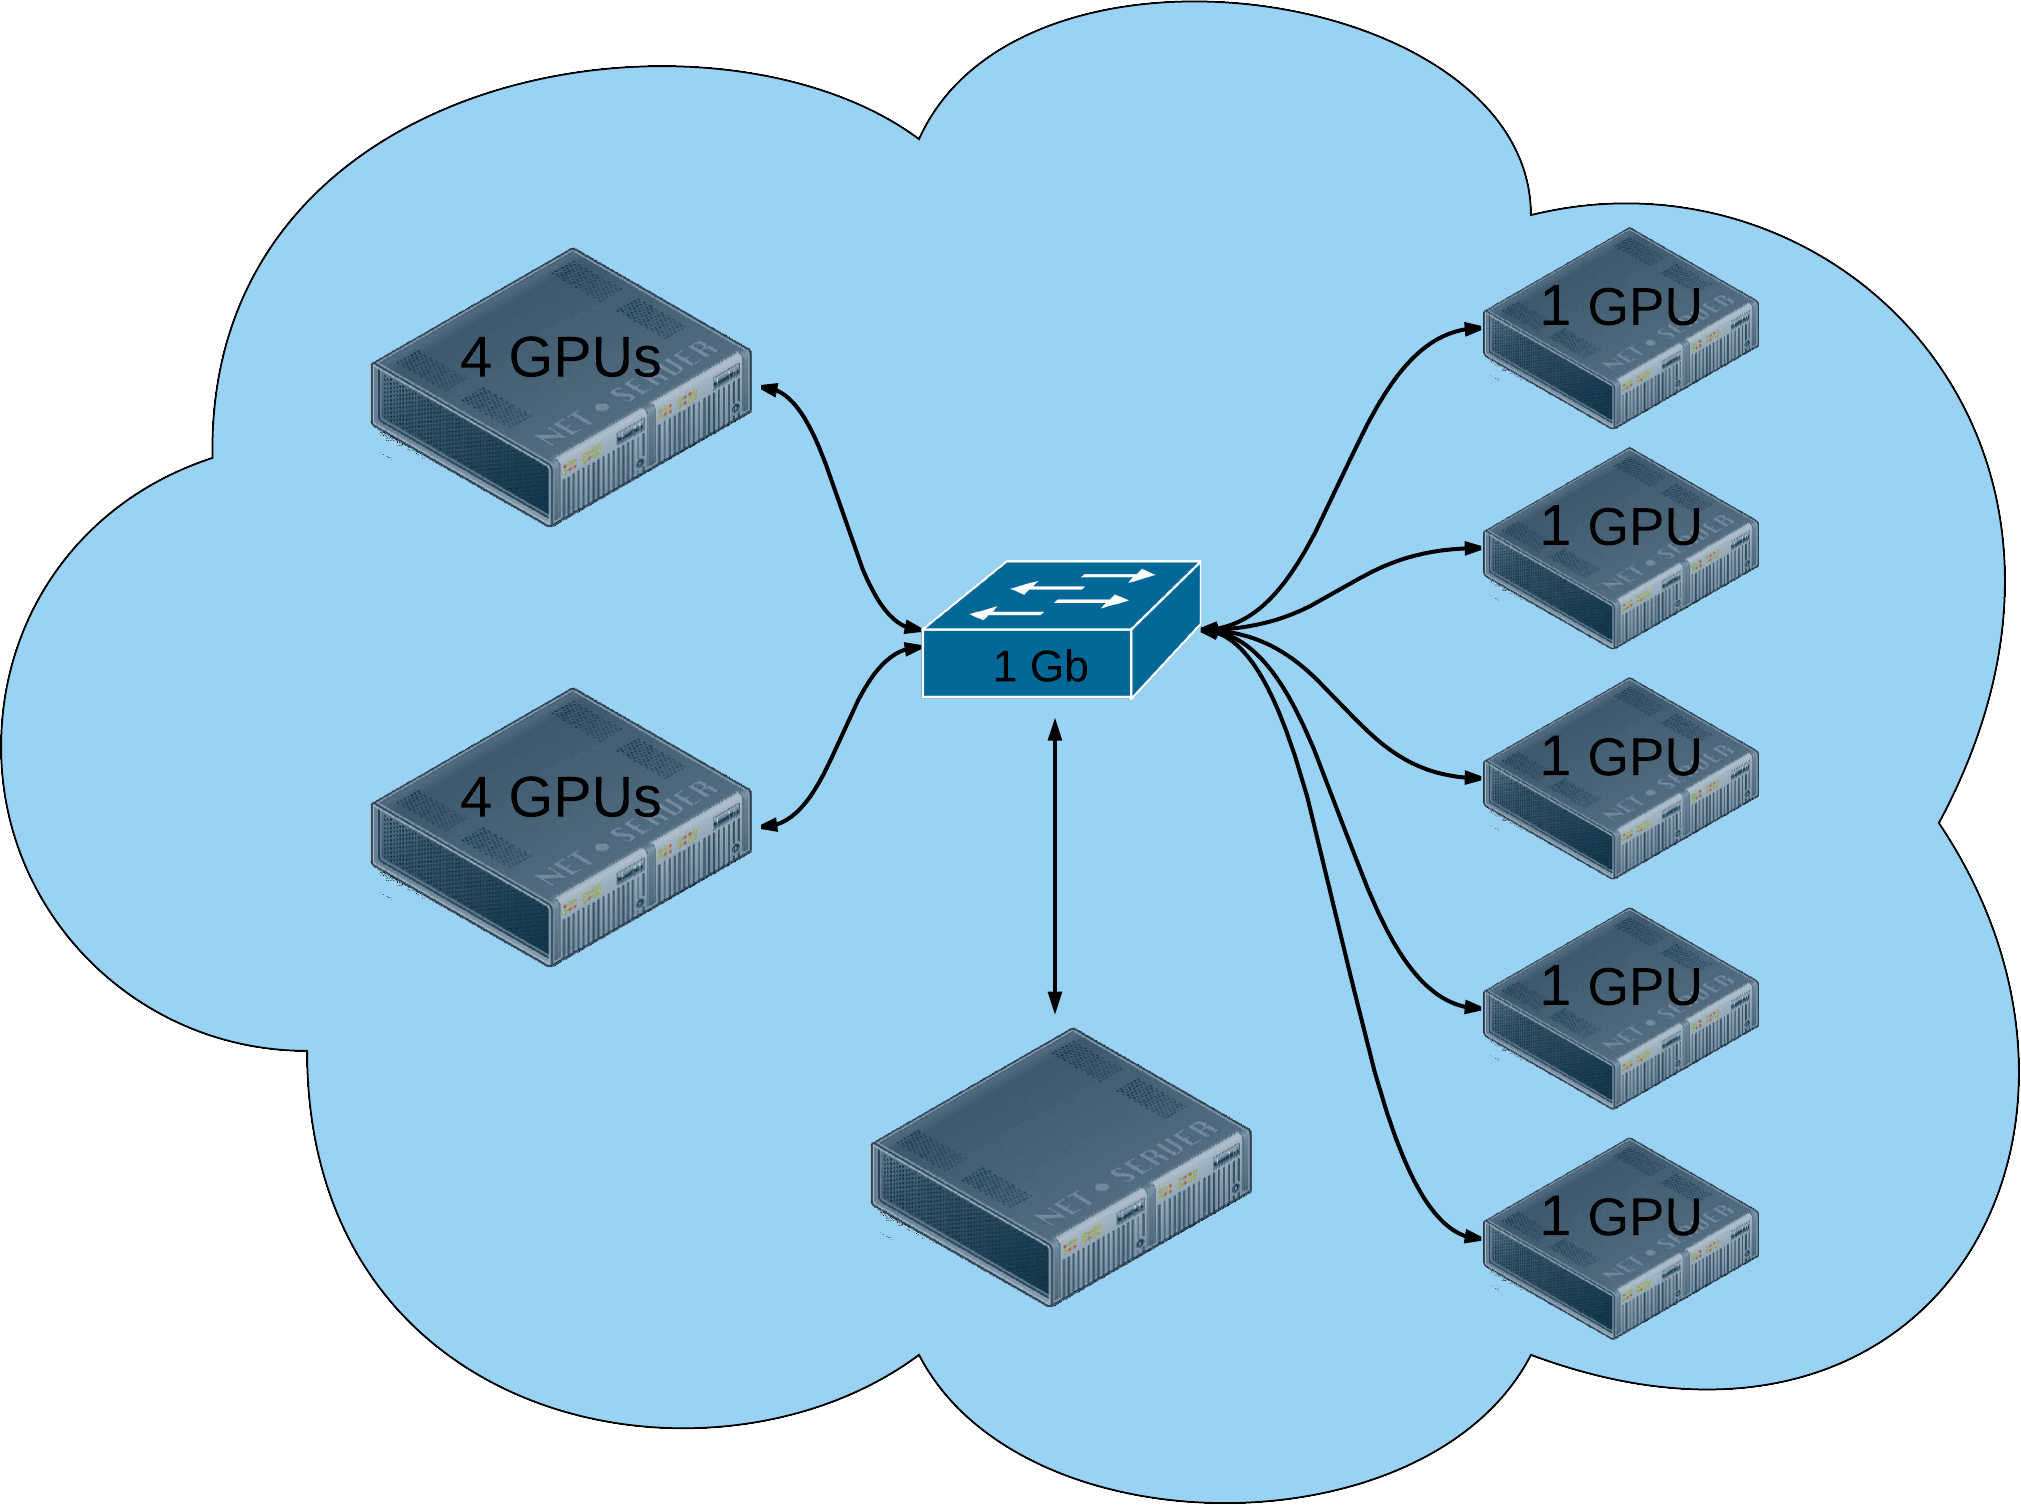
\includegraphics[width=0.31\linewidth]{images/aws1.png}
\label{subfig:aws3}}
\caption{Different configurations where an AWS instance acting as a client is using several remote GPUs.}
\label{fig:aws}
\end{figure*}

Once the scenarios are configured from the point of view of hardware, 
the {rCUDA} software needs to be installed in order to add 
the required flexibility to the system. So, the {rCUDA} server has been 
executed in the server nodes and the {rCUDA} libraries have been installed 
in the node that is acting as a client.

Moreover, with the aim to know the expected network bandwidth using 
a remote GPU, we have executed again the NVIDIA {\tt bandwidthtest} sample.
The results observed in the Table~\ref{table:bwtrcuda} shows how the bandwidth achieved is limited 
by the network.

\begin{table}[htb]
\renewcommand{\arraystretch}{1.3}
\caption{NVIDIA SDK {\tt bandwidthtest} execution transfering 32MB using pageable memory using {rCUDA}.}
\label{table:bwtrcuda}
\tabcolsep=0.09cm
\begin{center}\begin{tabular}{cccc}
Scenario &  Data Movement & Network & BandWidth \\ \hline \hline
A & Host to Device & High& 127 MB/s \\ \hline
A & Device to Host & High& 126 MB/s\\ \hline
B & Host to Device & 10 Gb& 858 MB/s\\ \hline
B & Device to Host & 10 Gb& 843 MB/s\\ \hline
\end{tabular}\end{center}\end{table}




\subsection{Experimental results}
In order to assess that GPU virtualization with AWS instances was working as expected, two applications were executed to analyze the results and their scalability.

The first of them was {\tt MonteCarloMultigpu} from NVIDIA SDK, launched with the default configuration ``scaling=weak'' which adjust the size of the problem depending on the number of accelerators.
The Figure~\ref{fig:mont-opt} depicts the options per second calculated by the application running on the scenarios of Figure~\ref{fig:aws} and on the instances with local GPUs. 
We have removed the results of the Scenario~\ref{subfig:aws2} for clarity ought to they are exactly the same that the obtained from Scenario~\ref{subfig:aws3} up to 8 GPUs. 
In other words, we could state that the results until the 8th GPU would correspond to the Scenario~\ref{subfig:aws2} and thereafter to the Scenario~\ref{subfig:aws3}.
Hence, in this particular case, rCUDA (using remote GPUs) is performing better than CUDA (with its local GPUs) due to rCUDA loads the libraries when its daemon starts.
However, even with rCUDA we can see differences in the results between booth scenarios. We determined that the Scenario~\ref{subfig:aws1} could increase the throughput because
unlike the other setups the GPUs are not sharing the PCI bus with other devices, as it happens in the 4-GPU instances.
% \begin{figure}[!t]
%   \centering
%   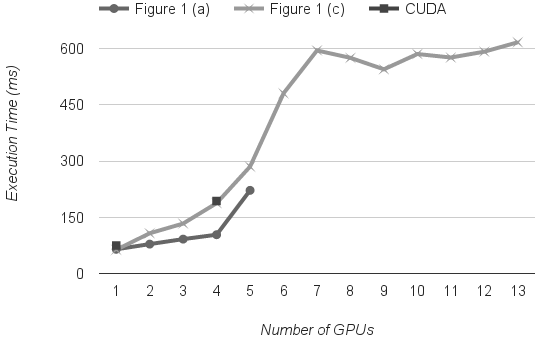
\includegraphics[width=\linewidth]{images/aws-mont2.png}
%   \caption{Montecarlo execution time}
%   \label{fig:mont-exe}
% \end{figure}
\begin{figure}[htb]
  \centering
  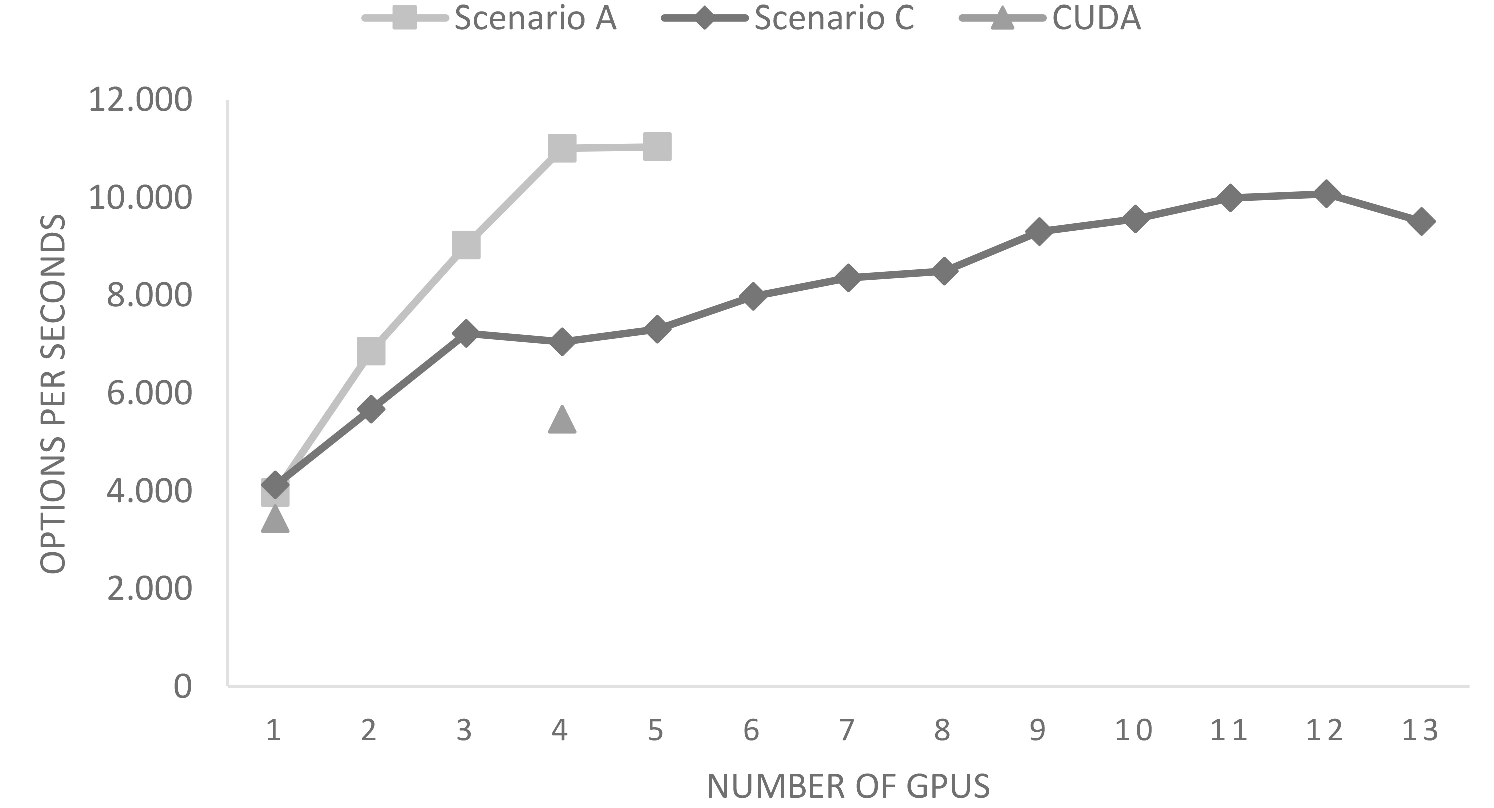
\includegraphics[width=\linewidth]{images/mont.pdf}
  \caption{NVIDIA SDK {\tt MonteCarloMultiGPU} execution using local and remote GPUs.}
  \label{fig:mont-opt}
\end{figure}

The other application, LAMMPS\footnote{\url{http://lammps.sandia.gov}}, is a classical molecular dynamics simulator that can be applied at the atomic, meso, or continuum scale. 
From the implementation perspective, this multi-process application employs at least one GPU to host its processes, but can benefit from the use of multiple GPUs.
The Figure shows that running this application using remote GPUs does not offer any advantage in front of original CUDA. 
Furthermore, for the execution on remote GPUs, can be seen a little difference between both networks, the ``High'' network performs worse than ``10 Gb'' network.
Thus, if we compare the results of a LAMMPS execution with a larger problem (see Figure), although CUDA continues performing better, the interesting point is the execution time on remote GPUs. 
They are almost the same even with different networks what means that the transfers are making the interconnection network the bottleneck, and enlarging the problem size
pays off the drawback of a slower network.

\begin{figure}[htb]
\centering
\subfigure[Run size = 100.]{%
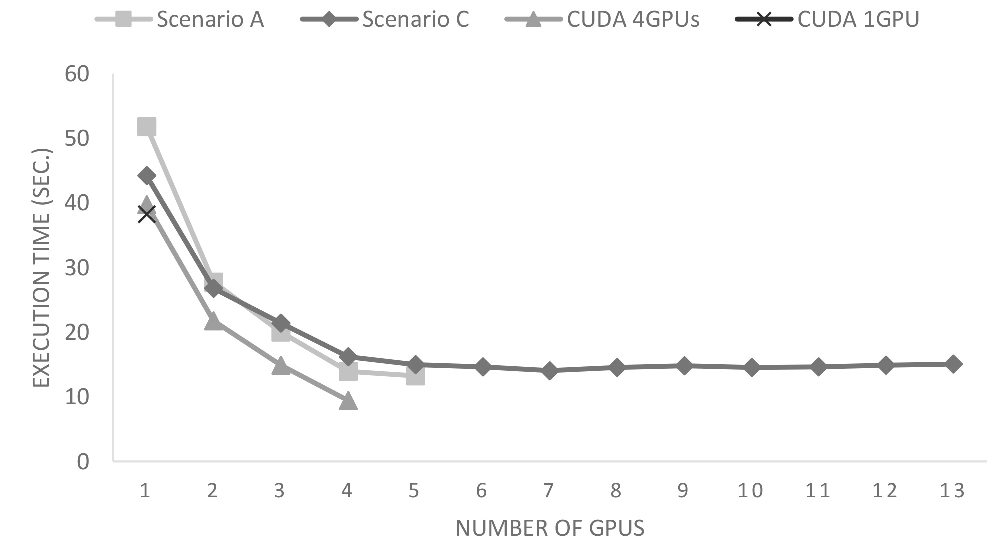
\includegraphics[width=\linewidth]{images/lammps1.pdf}
\label{subfig:lammps1}}
\quad
\subfigure[Run size = 2000.]{%
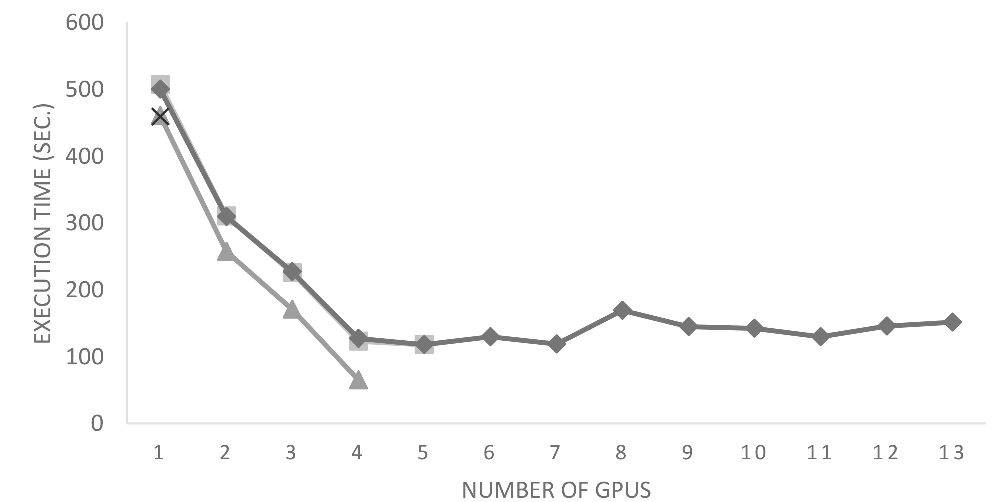
\includegraphics[width=\linewidth]{images/lammps2.pdf}
\label{subfig:lammps2}}
\caption{Execution time of LAMMPS.}
\label{fig:lammps}
\end{figure}

\subsection{Discussion}
Flexibility and economical expenses

\section{\uppercase{GPGPU Shared Service in OpenStack}}
In this section all the work related to OpenStack that has been done is explained, from the development of an external module to handle remote GPUs to the physical setup and its testing.

Version de open stack con la que se trabaja y tipo de instalacion ya que está toda en un nodo...

\subsection{Managing remote GPUs with OpenStack}
The main idea is to move from the original Openstack architecture (see Subfigure~\ref{subfig:os-orig}) to a solution where a new shared service takes part into the architecture and is responsible for all related to GPU accelerators (see Subfigure~\ref{subfig:os-mod}).
This new service would bring more flexibility when managing GPUs and new working modes for GPGPU computation in the Cloud.
As it is shown in Figure~\ref{fig:internal}, we have altered the OpenStack original Dashboard with a new parser, 
which split the HTTP query in order to make use of both, the GPGPU API for everything related to GPUs, and the nova API for the rest of the computation. 
The new GPGPU Service has brought a new feature which brings more flexibility when managing GPUs, from now on, we can create ``GPU-pools''. 
A ``GPU-pool'' is a set of independent GPUs (logically disattached from the nodes) that can be assigned to one or more instances.

\begin{figure}[htb]
  \centering
  \subfigure[Original in version XXXXXXXXXXXXXXXXXXXXXX]{
    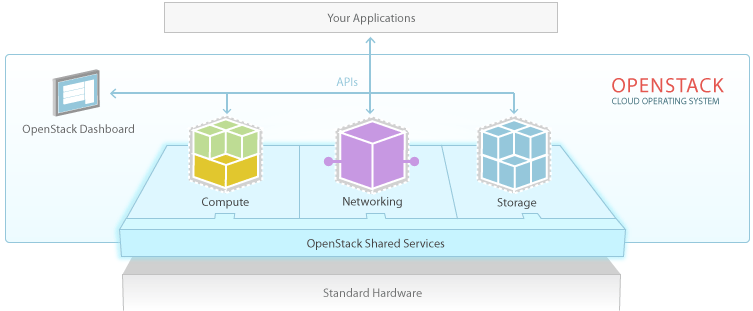
\includegraphics[width=\linewidth]{images/os-orig.png}
    \label{subfig:os-orig}
   }
   \quad
  \subfigure[With GPGPU developed module]{
    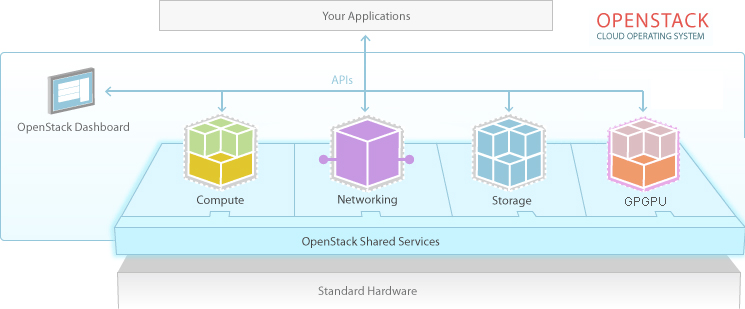
\includegraphics[width=\linewidth]{images/os1.jpg}
    \label{subfig:os-mod}
   }
  \caption{Openstack Architecture}
  \label{fig:os}
\end{figure}

\begin{figure}[htb]
  \centering
  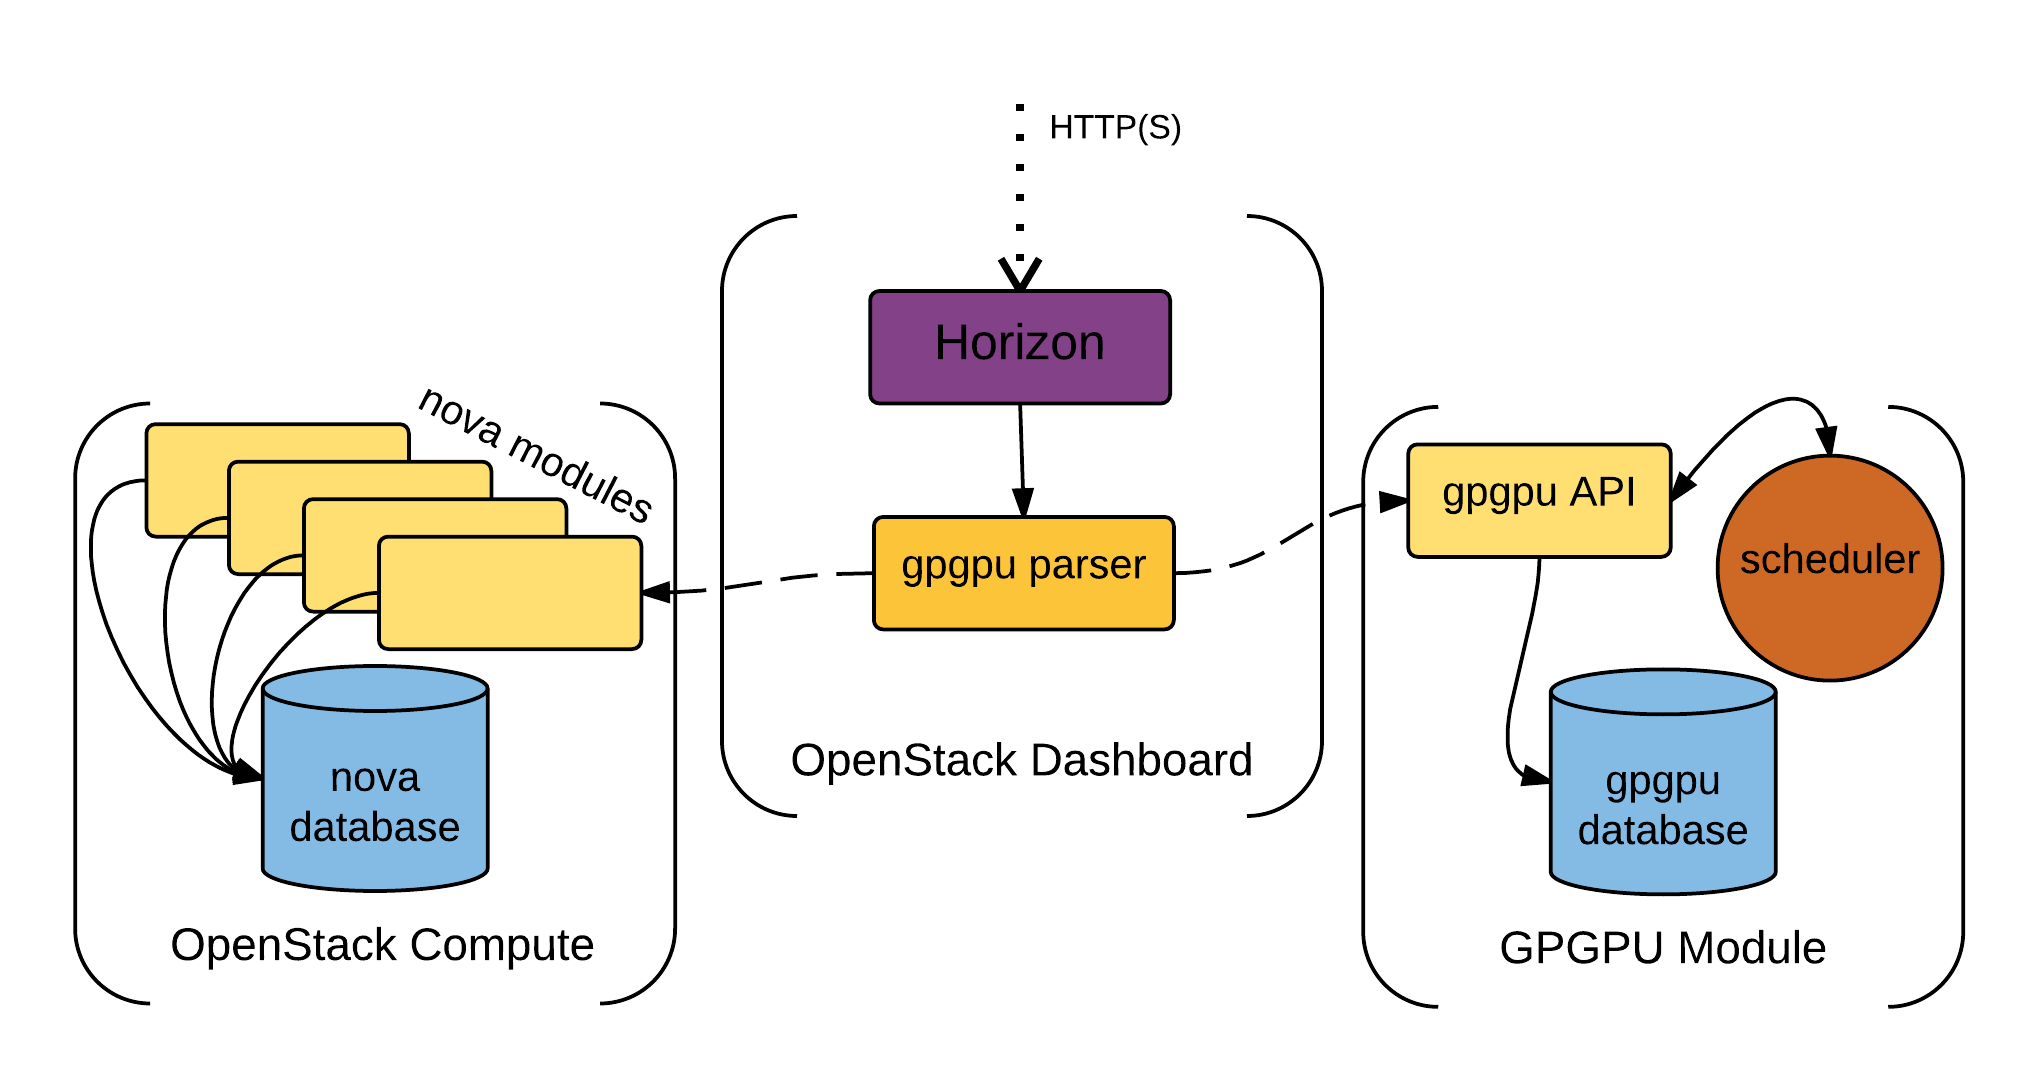
\includegraphics[width=\linewidth]{images/os2.png}
  \caption{Internal Communication among modules.}
  \label{fig:internal}
\end{figure}

Thanks to the modular approach of the GPGPU Service, the Nova Project has not been modified and the tool could be easily ported to other Cloud Computing solutions.

\subsection{Working Modes}
The developed module will allow the users to create any of the following scenarios (see Figure~\ref{fig2}). 
The users are given two configuration options to decide whether a physical GPU will be completely allocated for an instance (first column) or the instance will address a partition of the GPU as if it were a device (second column).
We refer to this as the ``mode'' and the possible values for this parameter are: ``exclusive'' or ``shared''. 
Let us suppose to have 4 GPU devices in the cluster (no matter where they were hosted, neither if they were in the same server). 
A well illustrated example of those scenarios can be seen in the first row of the  Figure~\ref{fig2}.
So, while in ``exclusive'' mode the instance is monopolizing all the GPUs, in the ``shared'' mode the GPUs have been partitioned. 
As a result of halving the GPU memory of the accelerators, the instance will be able to work with up to 8 GPUs.

Moreover, the users are also responsible for deciding whether a GPU (or a pool) will be assigned to other instances. 
This behaviour is refereed as ``scope'' and determines that a group of instances is logically connected to a pool of GPUs.
Working with ``public scope'' (second row of Figure~\ref{fig2}) means that the GPUs of a pool can be used simultaneously by all the instances linked to it.
Again, the GPU pool can be made of ``exclusive'' GPUs or ``shared''.

\begin{figure}[htb]
  \centering
  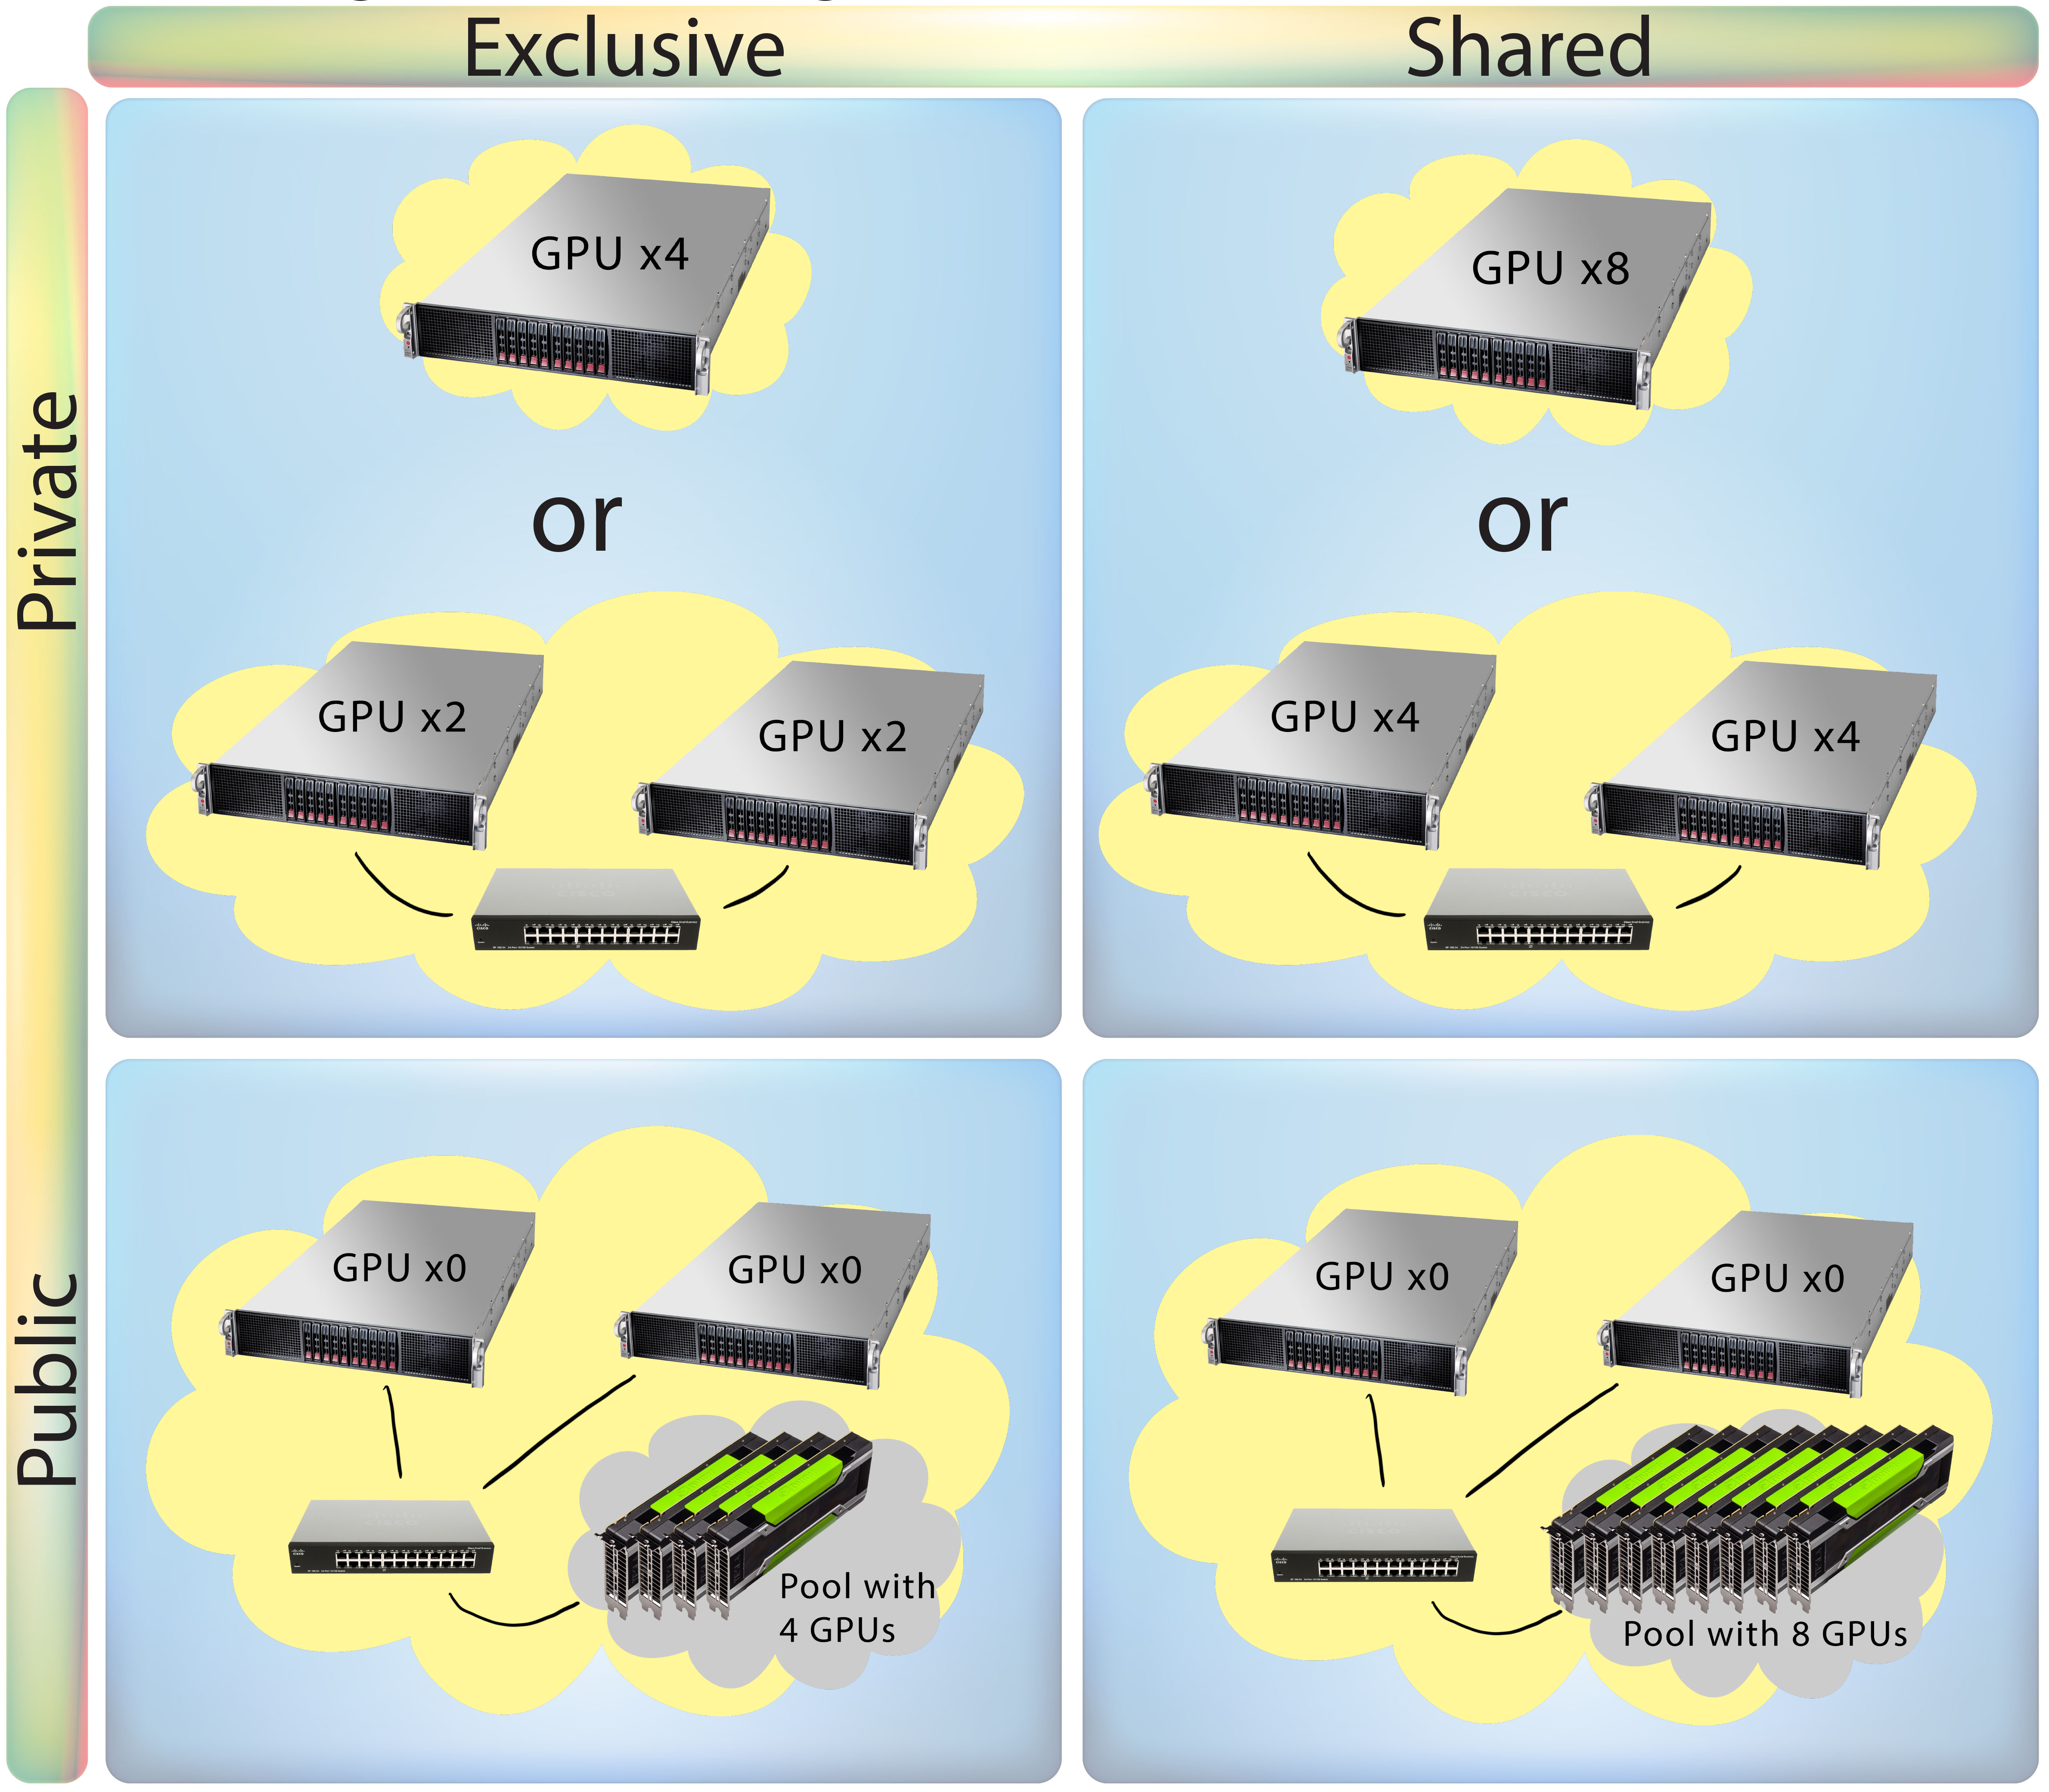
\includegraphics[width=.5\textwidth]{images/workingmodes.jpg}
  \caption{Examples of working modes.}
  \label{fig2}
\end{figure}

\subsection{User Interface}
Several modifications have been planned in the OpenStack Dashboard in order to deal with the new features.
First of all, the Instance Launch Panel should be provided with a new field, where the user could assign a existent GPU pool, create a new one or leave the instance without accelerators of this kind.
As soon as the option ``New GPU Pool'' had chosen, would appear the proper fields for the pool configuration (see Figure~\ref{fig:ui-launch}).
Furthermore, a new panel with the existent GPUs would display all the information related to GPUs (see Figure~\ref{fig:ui-rgpus}).

\begin{figure}[htb]
  \centering
  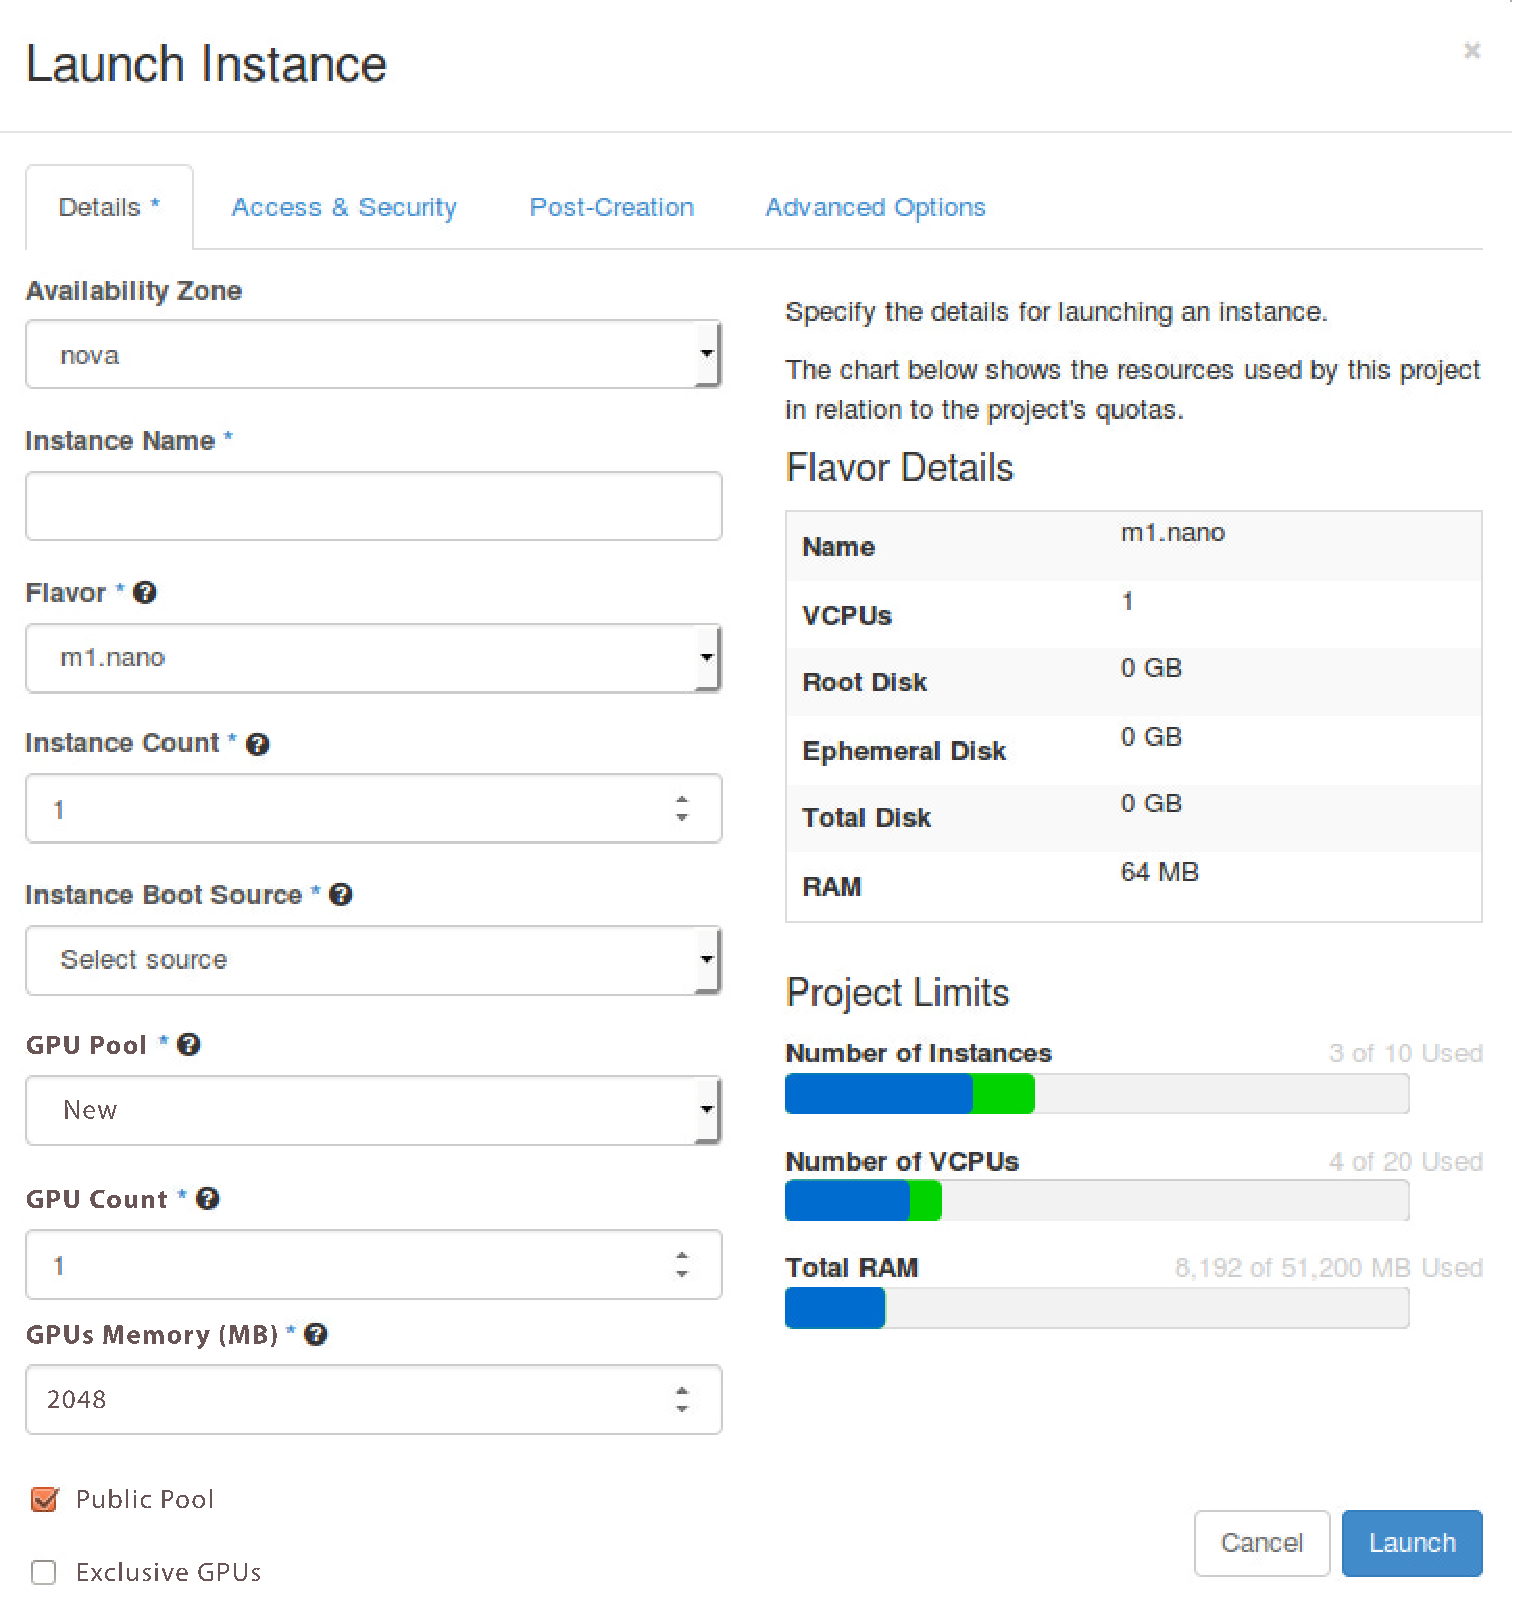
\includegraphics[width=\linewidth]{images/UI-launch.pdf}
  \caption{Launching Instances and assigning GPUs.}
  \label{fig:ui-launch}
\end{figure}
  
\begin{figure}[htb]
  \centering
  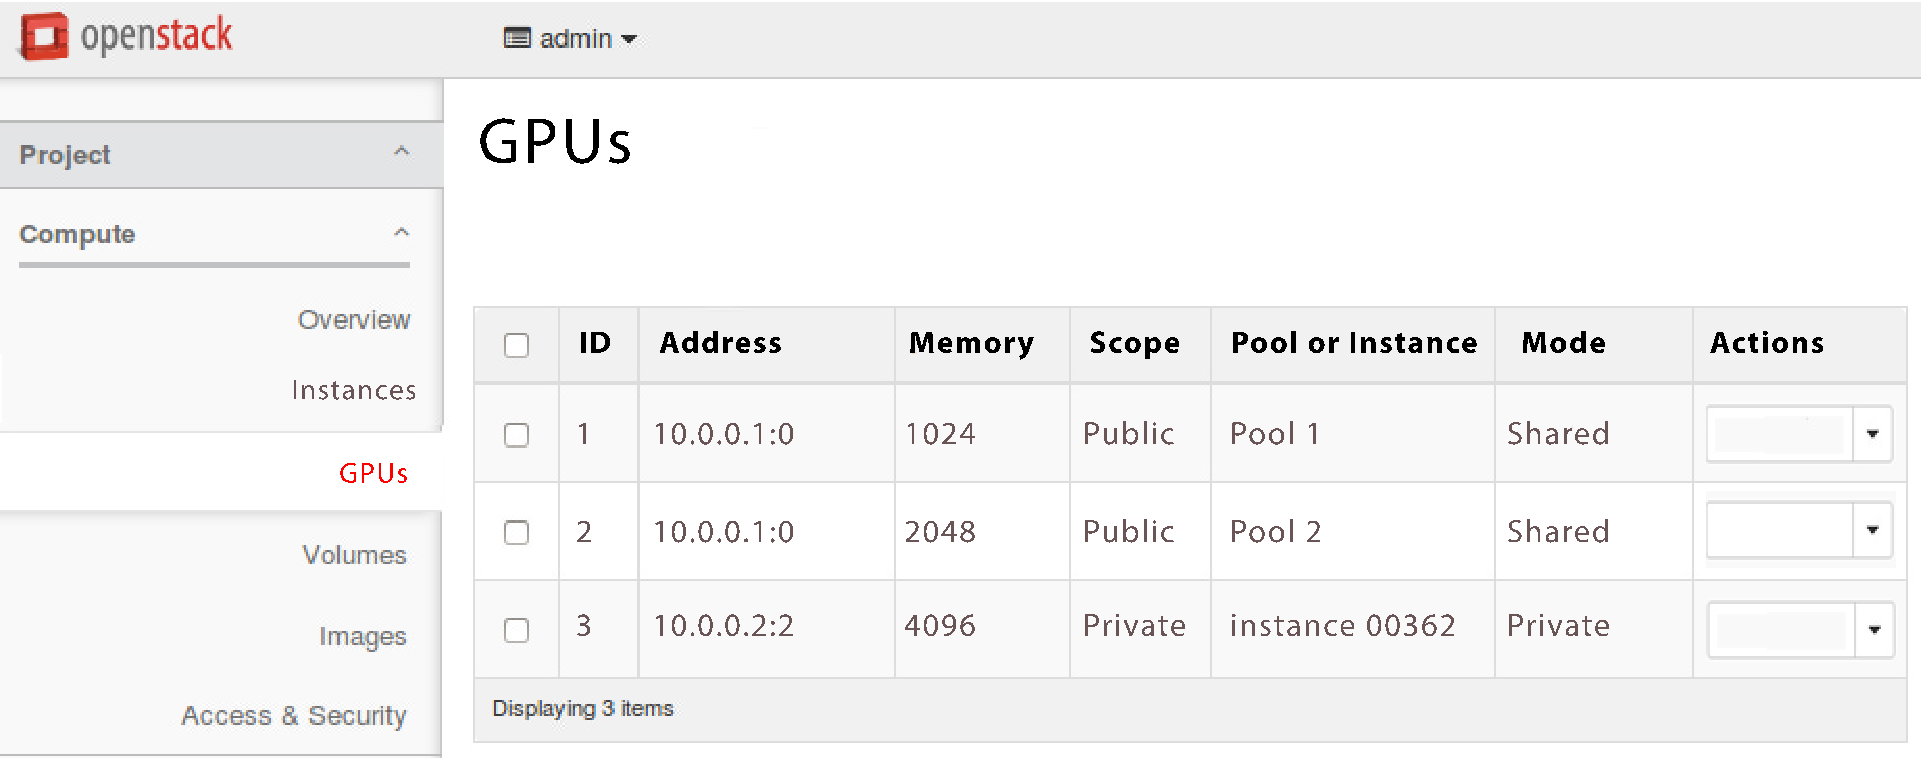
\includegraphics[width=\linewidth]{images/UI-rgpus.pdf}
  \caption{GPU Information Panel.}
  \label{fig:ui-rgpus}
\end{figure}

\subsection{Experimental Results}
The test were executed on a 5-node cluster where a machine
equipped with a Intel Xeon E7420 quadcore processor at
2.13 GHz, and 16 Gbytes of DDR2 RAM memory at 667
MHz, was guest host for the VMs. While the other 4 nodes
were auxiliary servers with a Tesla C1090 GPU each one. 
In the software stack the testbed system operates a
Centos 6.6; the cloud platform is deployed by OpenStack; and
the GPUs use CUDA 6.5. The GPU virtualization support is
based on rCUDA v5.0.

We have designed 6 different set-ups which can be divided
in 2 groups: “Exclusive GPUs” and “Shared GPUs”. The
“Exclusive” mode will provide, at most, 4 accelerators. Whilst
the number of available GPU in “Shared” mode will depend
on the partition size. In this particular case, we have halved
the memory, so we can use up to 8 GPUs. For each group, we
have deployed virtual clusters of 1, 2 and 3 nodes where will
run the processes of the application. The instances are based
on the flavor “m1.medium” which determines VM of 2 cores
and 4096 MB of memory.

MCUDA-MEME~\cite{Liu2010} has been the application executed with
different configurations in order to test the set-ups. MCUDA-
MEME is GPGPU MPI application, so the number of GPUs
will determine the number of executable processes.
The Figure~\ref{fig3} shows and compares the execution time of
the application with different configurations over different set-
ups. We can determine that with 1 node, the performance is
lower, with 2 and 3 is quite similar, though. Hence, the greatest
difference can be appreciated between modes, where the
highest performance is achieved by sharing the accelerators.

\begin{figure}[htb]
  \centering
  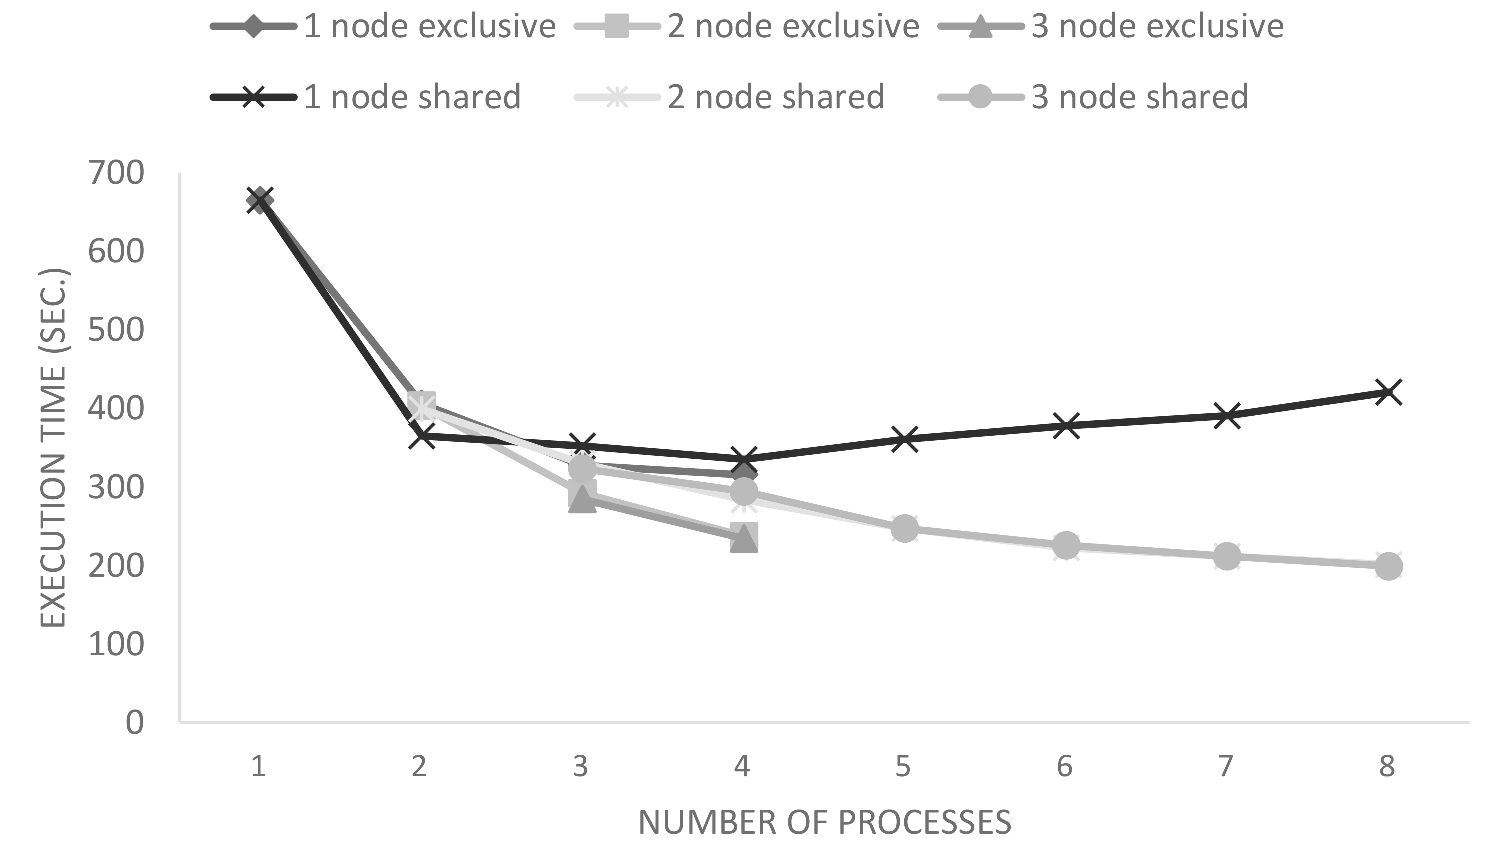
\includegraphics[width=\linewidth]{images/mcudameme-os.pdf}
  \caption{Scalability results of executing MCUDAMEME with a different number of MPI processes}
  \label{fig3}
\end{figure}

\section{\uppercase{Discussion}}
\label{sec:discussion}
-Volver a hacer un resumen
-posibles futuras aplicaciones (lab)
-pruebas con otros proveedores o con otras plataformas (azure)

\section{\uppercase{Conclusions}}
\label{sec:conclusions}


\section{\uppercase{Future work}}
\label{sec:future}


\section*{\uppercase{Acknowledgements}}
The authors would like to thank the IT members of the department Vicente Roca and Gustavo Edo for their help.

The researchers were supported by Universitat Jaume I research project (P11B2013-21), project
TIN2011-23283 and~FEDER.

\bibliographystyle{apalike}
{\small
\bibliography{paper}}


\end{document}
